
Если $f(x)$ непрерывна в~точке (определение \ref{ot})\footnote{Вот он, единственный пока что недостаток этих лекций.}$a$, то $f(x)$ ограничена в~точке $a$ (локально ограничена, рис. \ref{pogr}).

\begin{figure}[htbp]\centering
    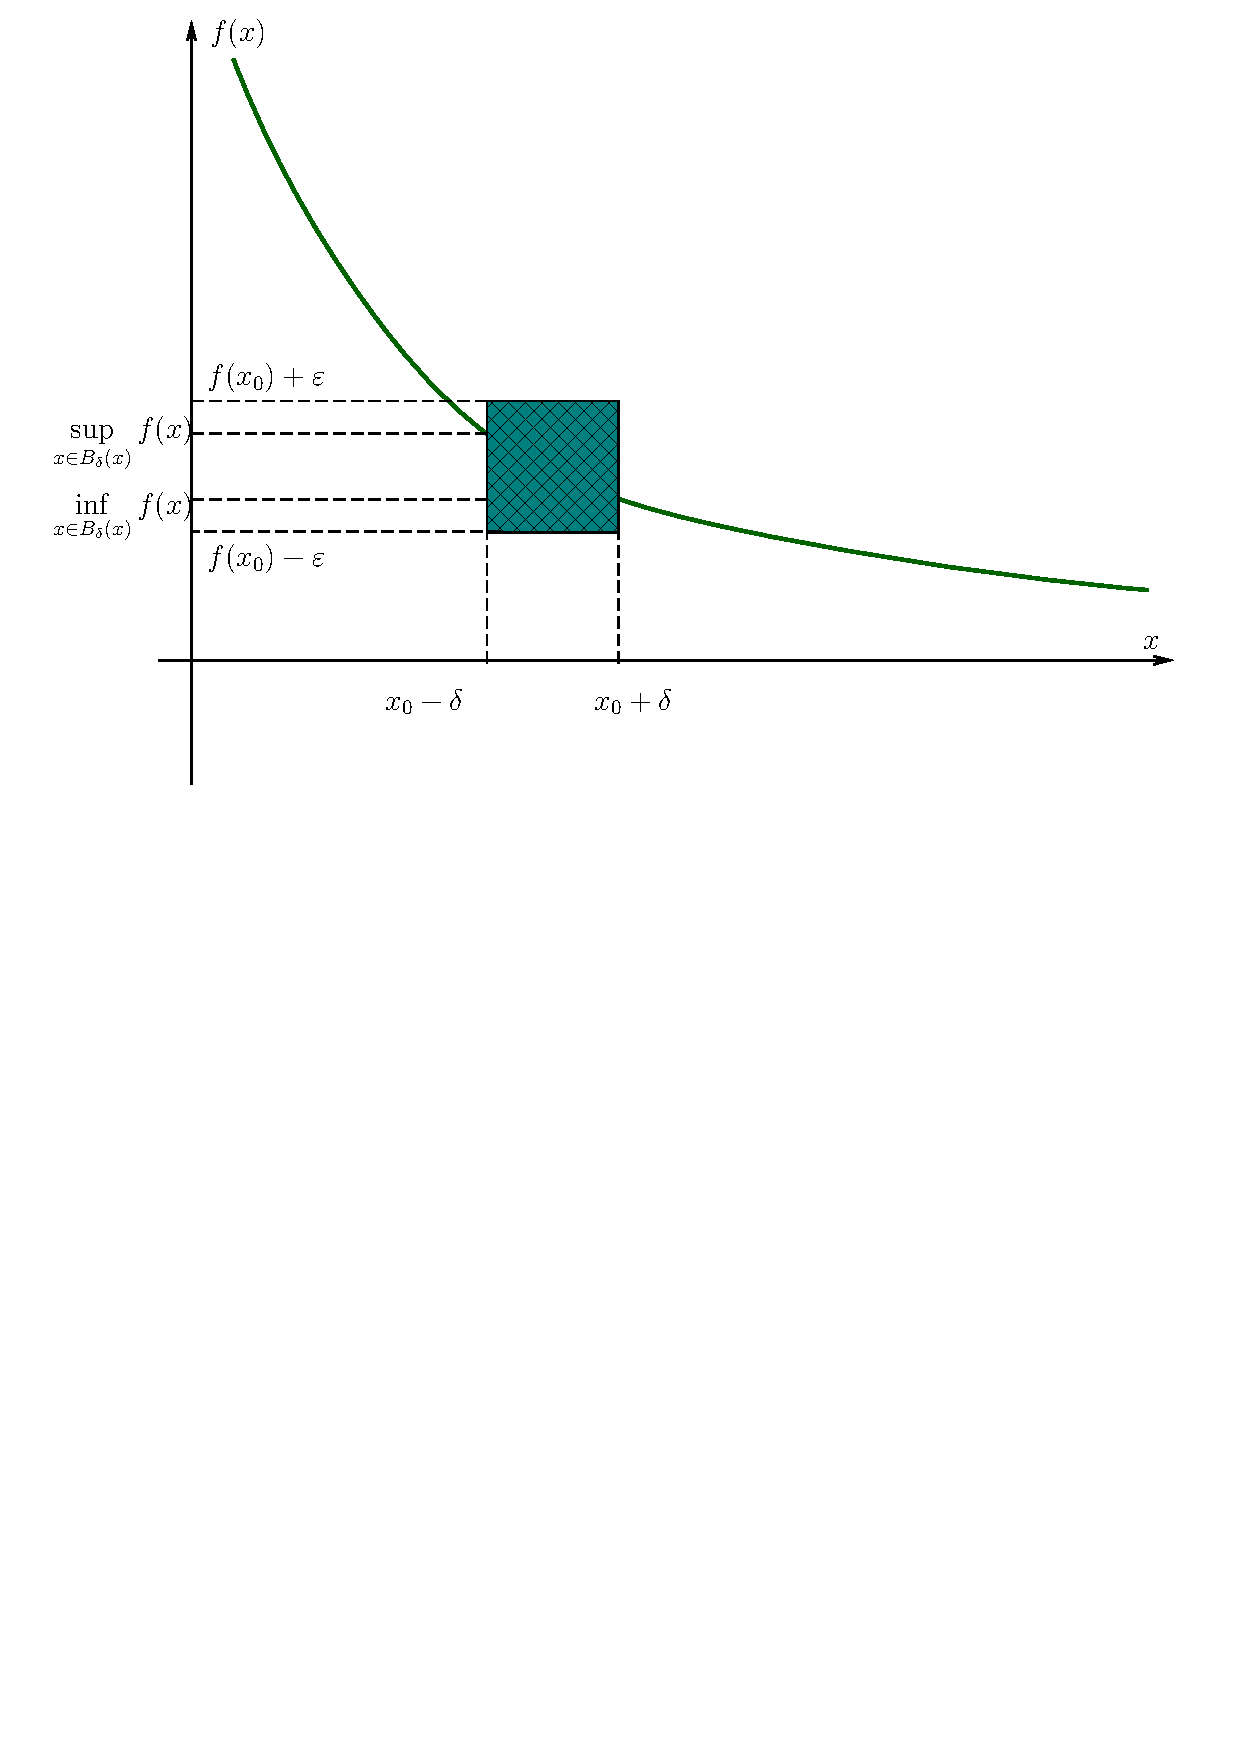
\includegraphics[height=8cm]{img/final/galat/ogr.pdf}\\ \caption{Непрерывна в~$x_0$ $\hm{\imp}$ ограниченна в~$x_0$}\label{pogr}
\end{figure}
